\documentclass[11pt]{article}
\usepackage[margin=1in]{geometry}
\usepackage{amsmath,amssymb,amsfonts,bm,mathtools}
\usepackage{booktabs,longtable,array}
\usepackage{siunitx}
\usepackage{graphicx,xcolor,enumitem,microtype}
\usepackage{hyperref,cleveref}
\usepackage{tikz}
\usetikzlibrary{arrows.meta,positioning,calc,shapes.geometric}
\hypersetup{colorlinks=true,linkcolor=blue,citecolor=blue,urlcolor=blue}
\newcommand{\dd}{\mathrm{d}}
\newcommand{\kb}{k_{\mathrm B}}
\newcommand{\ii}{\mathrm i}
\newcommand{\vv}{\mathrm v}
\newcommand{\bJ}{\bm{J}}
\newcommand{\bD}{\bm{D}}
\newcommand{\bP}{\bm{P}}
\newcommand{\beps}{\bm{\varepsilon}}
\newcommand{\bsigma}{\bm{\sigma}}
\newcommand{\bx}{\bm{x}}
\newcommand{\bh}{\bm{h}}
\newcommand{\bn}{\bm{n}}
\newcommand{\bb}{\bm{b}}
\newcommand{\bxi}{\bm{\xi}}
\newcommand{\cG}{\Gamma}
\newcommand{\cO}{\Omega}

\title{\textbf{Finite-Loop Point-Defect Transport in Irradiated $\alpha$-Zirconium}\\
A Unified Continuum--Atomistic Formulation Connecting Woo's Elastic Bias Theory and Atomistic Thermal-Drift Capture}
\author{}
\date{}

\begin{document}
\maketitle

\begin{abstract}
A finite dislocation loop in irradiated $\alpha$-zirconium is not merely a geometrical sink. Its elastic field changes both the equilibrium free energy of a mobile point defect and the migration barrier through the saddle-point configuration. Classical continuum treatments usually retain only an isotropic defect--loop interaction and consequently predict nearly the same bias for vacancy- and interstitial-type loops of equal size. Woo showed that anisotropy of the point-defect elastic dipole tensor at the migration saddle point breaks this symmetry and produces an intrinsic bias differential between vacancy and interstitial loops. More recently, March-Rico and Wirth obtained loop-character-dependent capture directly from atomistic binding-energy maps in $\alpha$-Zr and showed that thermal-drift capture can favor same-type defects.

The formulation developed here combines these ideas in a finite-loop transport problem. The loop is represented explicitly in three dimensions; its strain field is obtained from anisotropic HCP elasticity or a dislocation-dynamics solver; equilibrium and saddle-point defect energies are represented by elastic dipole tensors, atomistic energy maps, or a matched hybrid of both; local jump rates are constructed from transition-state theory; and the resulting position-dependent diffusion tensor is coupled to a drift--diffusion equation. The total point-defect flux into the finite loop directly defines the capture rate, sink strength, bias factor, and loop growth rate. Finite-element, finite-volume, kinetic Monte Carlo, and multiscale implementation strategies are described, together with verification tests and a practical computational workflow for $\alpha$-Zr.
\end{abstract}

\tableofcontents
\newpage

\section{Physical objective}
The objective is to calculate, without prescribing an empirical bias factor, the four finite-loop capture rates
\begin{equation}
K_{\ii,a_I},\qquad K_{\vv,a_I},\qquad K_{\ii,a_V},\qquad K_{\vv,a_V}.
\end{equation}
Using Woo's convention,
\begin{equation}
B_{a_I}=1-\frac{Z_{\vv,a_I}}{Z_{\ii,a_I}},\qquad
B_{a_V}=1-\frac{Z_{\vv,a_V}}{Z_{\ii,a_V}}.
\end{equation}
The principal question is whether the experimentally relevant regime
\begin{equation}
\boxed{B_{a_I}>0,\qquad B_{a_V}<0}
\end{equation}
emerges from the coupled effects of finite-loop elasticity, HCP diffusion anisotropy, equilibrium defect--loop binding, migration saddle-point anisotropy, near-core atomistic reconstruction, and actual loop geometry. Woo identified this as a possible intrinsic-bias regime and discussed zirconium as a candidate material \cite{Woo1982}; March-Rico and Wirth later obtained the same qualitative ``same-type'' tendency from atomistically calculated thermal-drift capture radii in $\alpha$-Zr \cite{MarchRicoWirth2023}.

\section{Finite-loop geometry and crystallography}
\subsection{Circular loop}
For a circular loop of radius $R_L$, center $\bx_0$, and orthonormal vectors $\bm e_1,\bm e_2$ spanning the loop plane,
\begin{equation}
\bn_L=\bm e_1\times\bm e_2,
\end{equation}
and
\begin{equation}
\cG_L:\quad \bx_L(\phi)=\bx_0+R_L(\bm e_1\cos\phi+\bm e_2\sin\phi),\qquad 0\le\phi<2\pi.
\end{equation}
The local line tangent is
\begin{equation}
\bxi(\phi)=\frac{\partial\bx_L/\partial\phi}{|\partial\bx_L/\partial\phi|}.
\end{equation}
For irradiation-induced $a$-loops in $\alpha$-Zr,
\begin{equation}
\bb_a=\frac13\langle11\bar20\rangle,\qquad |\bb_a|\simeq a,
\end{equation}
and the dominant habit-plane family is prismatic, commonly near $\{10\bar10\}$. The implementation should permit $\bn_L$ to be specified independently of $\bb_L$ so that first-order prism, second-order prism, and tilted habit planes can be represented.

\subsection{Signed loop character}
Define
\begin{equation}
s_L=\begin{cases}+1,&\text{interstitial loop},\\-1,&\text{vacancy loop},\end{cases}
\end{equation}
with a consistent loop-normal convention, and write
\begin{equation}
\bb_L=s_L\bb_0.
\end{equation}
For geometrically identical loops of opposite sign in linear elasticity,
\begin{equation}
\beps^{-L}(\bx)=-\beps^{+L}(\bx),\qquad \bsigma^{-L}(\bx)=-\bsigma^{+L}(\bx).
\end{equation}

\subsection{Core reaction surface}
Surround the dislocation line by a small reaction tube
\begin{equation}
\cG_c=\{\bx:d(\bx,\cG_L)=r_c\},
\end{equation}
where $d$ is shortest distance to the loop line. A species- and orientation-dependent $r_c$ can be used, but in the most fundamental calculation $r_c$ should remain a small core boundary and the long-range bias should emerge from the transport equations.

\section{Anisotropic elastic field of the finite loop}
For $\alpha$-Zr, use the full hexagonal stiffness tensor
\begin{equation}
\sigma_{ij}=C_{ijkl}\varepsilon_{kl}^{e},
\end{equation}
with independent constants $C_{11},C_{12},C_{13},C_{33},C_{44}$ and $C_{66}=(C_{11}-C_{12})/2$. Away from the core,
\begin{equation}
\partial_j\sigma_{ij}=0.
\end{equation}
The dislocation can be introduced through a Volterra cut, plastic distortion, eigenstrain, or anisotropic Green-function/Stroh representation \cite{HirthLothe,Mura}. The required output is
\begin{equation}
\boxed{\beps^L(\bx)=\beps^L(\bx;R_L,\bb_L,\bn_L,\mathbf C)}.
\end{equation}
Practical routes are: (i) anisotropic line-segment superposition, (ii) a DDD field evaluator, (iii) an eigenstrain/FEM elasticity solve, or (iv) an isotropic circular-loop benchmark. A non-singular core regularization is recommended when atomistic core corrections are not supplied explicitly.

\section{Point-defect energetics}
\subsection{Equilibrium elastic dipole}
For point-defect species $\alpha\in\{\ii,\vv\}$, define
\begin{equation}
P_{ij}^{g,\alpha}=-\frac{\partial E_f^\alpha}{\partial\varepsilon_{ij}}.
\end{equation}
To first order in strain,
\begin{equation}
\boxed{E_g^{\alpha L}(\bx)=-P_{ij}^{g,\alpha}\varepsilon_{ij}^{L}(\bx)}.
\end{equation}
For an isotropic dilatation center, $P_{ij}^{g,\alpha}=P_g^\alpha\delta_{ij}$ and the interaction reduces to hydrostatic coupling.

\subsection{Saddle-point elastic dipole}
For a thermally activated jump in direction $\hat{\bh}_k$, define the saddle dipole
\begin{equation}
\bP_k^{s,\alpha}=\bP^{s,\alpha}(\hat{\bh}_k),
\end{equation}
and
\begin{equation}
\boxed{E_s^{\alpha L}(\bx,\hat{\bh}_k)=-P_{ij}^{s,\alpha}(\hat{\bh}_k)\varepsilon_{ij}^{L}(\bx)}.
\end{equation}
Woo's 1982 theory emphasizes that anisotropy of $\bP^{s,\alpha}$ can break the vacancy-loop/interstitial-loop symmetry even within linear elasticity \cite{Woo1982}. Dederichs and Schroeder derived the corresponding anisotropic diffusion in stress fields from a microscopic lattice description \cite{DederichsSchroeder1978}.

\subsection{Local migration barrier}
Let $E_{m,0}^{\alpha k}$ be the unstrained barrier for jump $k$. Then
\begin{equation}
\boxed{E_m^{\alpha L}(\bx,\hat{\bh}_k)=E_{m,0}^{\alpha k}+E_s^{\alpha L}(\bx,\hat{\bh}_k)-E_g^{\alpha L}(\bx)}.
\end{equation}
This is the central bridge between Woo's saddle-point theory and an atomistically informed finite-loop calculation.

\subsection{External stress}
If external or microstructural strain is present, use
\begin{equation}
\beps^{\rm tot}=\beps^L+\beps^{\rm ext}
\end{equation}
in both equilibrium and saddle interactions. This permits local crystal-plasticity stress, grain-boundary stress, neighboring-loop fields, and network-dislocation stress to enter the capture calculation.

\section{Atomistic near-core energetics}
March-Rico and Wirth calculated point-defect binding-energy maps around interstitial $a$-loops, vacancy $a$-loops, and vacancy $c$-loops in $\alpha$-Zr using molecular statics \cite{MarchRicoWirth2023}. Write such an equilibrium map as
\begin{equation}
E_{g,\rm atom}^{\alpha L}(\bx).
\end{equation}
A direct test of Woo's mechanism additionally requires saddle maps
\begin{equation}
E_{s,\rm atom}^{\alpha L}(\bx,\hat{\bh}_k),
\end{equation}
obtained by NEB, dimer, or equivalent saddle-search calculations.

A matched elastic--atomistic representation is
\begin{equation}
E_{g,\rm hyb}=E_{g,\rm el}+w(d)(E_{g,\rm atom}-E_{g,\rm el}),
\end{equation}
\begin{equation}
E_{s,\rm hyb}=E_{s,\rm el}+w(d)(E_{s,\rm atom}-E_{s,\rm el}),
\end{equation}
with $w\to1$ near the core and $w\to0$ in the elastic far field. This avoids double counting.

\section{Discrete jump formulation}
For an allowed jump $\bh_k=h_k\hat{\bh}_k$, transition-state theory gives
\begin{equation}
\boxed{\Gamma_{\alpha k}^{L}(\bx)=\nu_{\alpha k}\exp[-\beta E_m^{\alpha L}(\bx,\hat{\bh}_k)]},\qquad \beta=(\kb T)^{-1}.
\end{equation}
For strict detailed balance, forward and reverse transitions should share the same physical saddle state. The lattice master equation is
\begin{align}
\frac{\partial C_\alpha(\bx,t)}{\partial t}
&=\sum_k\Big[\Gamma_{\alpha,-k}^{L}(\bx+\bh_k)C_\alpha(\bx+\bh_k,t)
-\Gamma_{\alpha,k}^{L}(\bx)C_\alpha(\bx,t)\Big]\\
&\quad+G_\alpha-R_\alpha.
\end{align}
This equation can be solved directly by lattice kinetic Monte Carlo or homogenized to a continuum transport equation.

\section{Continuum drift--diffusion formulation}
For a dilute defect population,
\begin{equation}
\mu_\alpha=\mu_\alpha^0+\kb T\ln\left(\frac{C_\alpha}{C_\alpha^{\rm ref}}\right)+E_g^{\alpha L}(\bx).
\end{equation}
Using an Onsager mobility tensor $\bm M_\alpha^L$,
\begin{equation}
\bJ_\alpha=-\bm M_\alpha^L C_\alpha\nabla\mu_\alpha.
\end{equation}
Defining $\bD_\alpha^L=\kb T\bm M_\alpha^L$ gives
\begin{equation}
\boxed{\bJ_\alpha=-\bD_\alpha^L(\bx)\left[\nabla C_\alpha+\beta C_\alpha\nabla E_g^{\alpha L}(\bx)\right]}.
\end{equation}
The local diffusion tensor is generated from the stressed jump network, schematically
\begin{equation}
\boxed{D_{\alpha,ij}^{L}(\bx)=\frac12\sum_k\Gamma_{\alpha k}^{\rm eff}(\bx)h_{k,i}h_{k,j}},
\end{equation}
with $\Gamma^{\rm eff}$ formed from forward/reverse rates in a detailed-balance-consistent manner.

Far from the loop, HCP diffusion has the form
\begin{equation}
\bD_\alpha^\infty=D_{\alpha,a}(\bm e_{a1}\otimes\bm e_{a1}+\bm e_{a2}\otimes\bm e_{a2})+D_{\alpha,c}\bm e_c\otimes\bm e_c.
\end{equation}
Thus the same calculation contains diffusion anisotropy difference (DAD), elastic drift, and saddle-point anisotropy.

If the diffusion time $\tau_D\sim L^2/D_\alpha$ is short relative to loop evolution, the quasi-steady problem is
\begin{equation}
\boxed{\nabla\cdot\left\{\bD_\alpha^L(\bx)\left[\nabla C_\alpha+\beta C_\alpha\nabla E_g^{\alpha L}\right]\right\}=0}.
\end{equation}
Four independent problems are solved for $(\ii,a_I)$, $(\vv,a_I)$, $(\ii,a_V)$, and $(\vv,a_V)$.

\section{Slotboom transformation}
Define
\begin{equation}
u_\alpha=C_\alpha\exp(\beta E_g^{\alpha L}).
\end{equation}
Then
\begin{equation}
\nabla C_\alpha+\beta C_\alpha\nabla E_g^{\alpha L}
=\exp(-\beta E_g^{\alpha L})\nabla u_\alpha,
\end{equation}
so
\begin{equation}
\boxed{\bJ_\alpha=-\underbrace{\bD_\alpha^L\exp(-\beta E_g^{\alpha L})}_{\bm A_\alpha(\bx)}\nabla u_\alpha}
\end{equation}
and
\begin{equation}
\boxed{\nabla\cdot[\bm A_\alpha(\bx)\nabla u_\alpha]=0}.
\end{equation}
This form removes the explicit convection-like drift term. If $\bD_\alpha^L$ is symmetric positive definite, the transformed equation is a variable-coefficient elliptic problem and is usually preferable for finite-element solution.

\section{Boundary conditions}
\subsection{Outer boundary}
For an isolated loop,
\begin{equation}
C_\alpha=C_\alpha^\infty\qquad\text{on }\cG_\infty.
\end{equation}
The boundary must be far enough from the loop that the integrated flux is insensitive to its location. For a periodic loop population, periodic or symmetry conditions may be used, with representative cell volume $V_{\rm cell}\simeq N_L^{-1}$.

\subsection{Perfect sink}
The simplest core condition is
\begin{equation}
C_\alpha=C_{\alpha,L}^{\rm eq}\qquad\text{on }\cG_c.
\end{equation}
For a pure sink-strength benchmark, $C_{\alpha,L}^{\rm eq}\to0$.

\subsection{Finite core reaction}
A more general radiation boundary condition is
\begin{equation}
\boxed{\bn_c\cdot\bJ_\alpha=\kappa_{\alpha L}(C_\alpha-C_{\alpha,L}^{\rm eq})\qquad\text{on }\cG_c},
\end{equation}
where $\bn_c$ points from the matrix into the sink. This permits partial reflection and avoids forcing all near-core kinetics into an arbitrary capture radius.

\subsection{Emission and detailed balance}
For loop evolution, $C_{\alpha,L}^{\rm eq}$ should be obtained from detailed balance using the free-energy change for adding/removing a point defect from the loop. This can include line tension, stacking-fault energy, external stress work, and chemical terms.

\section{Flux, capture coefficient, sink strength, and bias}
The net absorption rate of species $\alpha$ is
\begin{equation}
\boxed{\Phi_{\alpha L}=\int_{\cG_c}\bJ_\alpha\cdot\bn_c\,\dd A}.
\end{equation}
Define the single-loop rate constant
\begin{equation}
K_{\alpha L}=\frac{\Phi_{\alpha L}}{C_\alpha^\infty-C_{\alpha,L}^{\rm eq}}.
\end{equation}
For one loop in a cell of volume $V_{\rm cell}$,
\begin{equation}
k_{\alpha L}^2=\frac{K_{\alpha L}}{D_\alpha^{\rm ref}V_{\rm cell}}.
\end{equation}
The corresponding mean-field sink loss is
\begin{equation}
\left.\frac{\partial C_\alpha}{\partial t}\right|_L=-D_\alpha^{\rm ref}k_{\alpha L}^2(C_\alpha-C_{\alpha,L}^{\rm eq}).
\end{equation}
Using Woo's convention,
\begin{equation}
\boxed{B_L=1-\frac{k_{\vv L}^2}{k_{\ii L}^2}}.
\end{equation}
March-Rico and Wirth use $B_L^{\rm MR}=Z_{\ii,L}/Z_{\vv,L}-1$, related by
\begin{equation}
B_L^{\rm Woo}=\frac{B_L^{\rm MR}}{1+B_L^{\rm MR}}.
\end{equation}

\section{Finite-loop growth law}
For an ideal prismatic loop,
\begin{equation}
N_L\simeq\frac{\pi R_L^2 b_n}{\Omega},\qquad b_n=|\bb_L\cdot\bn_L|.
\end{equation}
With signed defect content $q_L=s_LN_L$,
\begin{equation}
\dot q_L=\Phi_{\ii L}-\Phi_{\vv L},
\end{equation}
so
\begin{equation}
\boxed{\dot R_L=\frac{\Omega}{2\pi R_Lb_ns_L}(\Phi_{\ii L}-\Phi_{\vv L})}.
\end{equation}
Thus an interstitial loop grows when SIA influx dominates, while a vacancy loop grows when vacancy influx dominates. Cluster absorption/emission can be added to the right-hand side.

\section{Relation to earlier theories}
\subsection{Geometrical sink}
If $E_g=E_s=0$, then
\begin{equation}
\nabla\cdot(\bD_\alpha^\infty\nabla C_\alpha)=0,
\end{equation}
and only geometry and bulk diffusion anisotropy remain.

\subsection{Classical isotropic elastic bias}
If
\begin{equation}
\bP^{g,\alpha}=P_g^\alpha\bm I,\qquad \bP^{s,\alpha}=P_s^\alpha\bm I,
\end{equation}
the interaction is dominated by isotropic/hydrostatic coupling. In the harmonic limit, equal-sized vacancy and interstitial loops have nearly the same intrinsic bias. Woo's 1981 effective-medium calculation is a finite-loop implementation of this class of theory \cite{Woo1981}.

\subsection{Woo 1982 saddle-point anisotropy}
Woo allowed $\bP^{s,\alpha}$ to be anisotropic and showed that the defect/loop interaction is then generally non-harmonic. Reversing loop character changes the sign of the shape-sensitive term, giving
\begin{equation}
B_{a_I}\ne B_{a_V}.
\end{equation}
In the infinitesimal-loop, dilute-sink limit, Woo obtained analytic reaction radii and bias expressions in terms of saddle-point dipole eigenvalues \cite{Woo1982}. The finite-loop calculation should reduce toward this limit under the same assumptions.

\subsection{March-Rico--Wirth atomistic thermal drift}
March-Rico and Wirth calculated relaxed defect binding-energy maps around finite Zr loops. Spontaneous capture favored SIAs for all loops, whereas thermal-drift capture produced a same-type tendency correlated with local loop stress \cite{MarchRicoWirth2023}. Their later cluster-dynamics work showed that thermal-drift capture radii stabilize vacancy $a$-loop growth and permit concurrent vacancy/interstitial $a$-loop evolution \cite{MarchRicoBlondelWirth2025}. The present framework replaces a single thermal-drift capture radius by an explicit transport solution through the full energy and mobility landscapes.

\section{Recommended hierarchy of models}
A useful decomposition is:
\begin{description}
\item[Model G: Geometry only.] $E_g=E_s=0$; retain HCP bulk diffusion anisotropy.
\item[Model I: Isotropic elasticity.] Use isotropic equilibrium and saddle dipoles.
\item[Model S: Woo saddle anisotropy.] Use anisotropic $\bP^s$ and equilibrium $\bP^g$ with continuum loop elasticity.
\item[Model B: Atomistic binding only.] Use atomistic $E_g(\bx)$ with bulk $\bD_\alpha^\infty$, but no position-dependent saddle correction.
\item[Model H: Hybrid.] Use atomistically corrected $E_g$ and $E_s$, matched to anisotropic continuum elasticity at long range.
\end{description}
Comparisons among these models isolate geometric, DAD, equilibrium-binding, saddle-point, and near-core contributions to the bias.

\section{Weak finite-element formulation}
Using the Slotboom variable,
\begin{equation}
\nabla\cdot(\bm A_\alpha\nabla u_\alpha)=0,
\qquad
\bm A_\alpha=\bD_\alpha^L e^{-\beta E_g^{\alpha L}}.
\end{equation}
For test function $v$ vanishing on Dirichlet boundaries,
\begin{equation}
\boxed{\int_{\cO}\nabla v\cdot\bm A_\alpha\nabla u_\alpha\,\dd V
-\int_{\partial\cO_N}v\,\bn\cdot\bm A_\alpha\nabla u_\alpha\,\dd A=0}.
\end{equation}
For a perfect-sink Dirichlet boundary, $u_\alpha$ is prescribed on $\cG_c$; for a Robin core reaction, the boundary term is replaced by the transformed reaction law. If $\bm A_\alpha$ is symmetric positive definite, the bilinear form is elliptic.

\section{Potential numerical solution methods}
\subsection{Finite elements: recommended primary method}
A 3-D unstructured tetrahedral FEM is the most flexible option because it naturally handles a toroidal core, anisotropic $\bD(\bx)$, anisotropic elasticity, Robin conditions, periodic boundaries, and local mesh refinement.

\paragraph{FEniCSx.} FEniCSx/DOLFINx is well suited because the weak form can be entered directly in UFL and solved with PETSc-based parallel linear algebra \cite{BarattaFEniCSx,AlnaesUFL}.

\paragraph{MOOSE.} MOOSE is attractive if the finite-loop transport calculation will later be coupled to mechanics, phase-field evolution, cluster dynamics, or other multiphysics models \cite{GastonMOOSE,PermannMOOSE}.

\subsection{Finite volume}
A conservative finite-volume method is attractive when exact local flux conservation is important. For strong drift, exponentially fitted/Scharfetter--Gummel fluxes can be used \cite{ScharfetterGummel}, especially when solving the untransformed equation.

\subsection{Boundary elements}
Boundary-element methods can be efficient for homogeneous transport coefficients and analytic drift potentials, but are much less attractive when $\bD_\alpha^L(\bx)$ varies strongly or atomistic energy maps are used.

\subsection{Kinetic Monte Carlo}
Lattice or object kinetic Monte Carlo provides an independent validation of the continuum closure and naturally retains discrete jump directions and saddle barriers \cite{MalerbaBecquartDomain2007}. It is, however, expensive for high-precision steady capture rates.

\subsection{Direct master-equation solve}
A sparse deterministic solve of the lattice master equation can bridge KMC and continuum FEM. It is useful for moderate atomistic/lattice domains because it preserves discrete jump topology without stochastic sampling noise.

\section{Mesh and domain design}
The domain must resolve a core scale of order angstroms and an outer scale of many nanometers. A practical strategy is:
\begin{enumerate}
\item construct a toroidal inner surface at $d=r_c$;
\item apply a highly refined boundary-layer mesh around the torus;
\item grow element size geometrically away from the loop;
\item refine where $|\nabla E_g|/(\kb T)$ or saddle corrections are large;
\item enlarge the outer domain until the integrated flux converges.
\end{enumerate}
Recommended convergence checks are
\begin{equation}
\left|\frac{\Phi(h/2)-\Phi(h)}{\Phi(h/2)}\right|<\epsilon_h,
\qquad
\left|\frac{\Phi(2R_\infty)-\Phi(R_\infty)}{\Phi(2R_\infty)}\right|<\epsilon_R.
\end{equation}

\section{Why the Zr problem is genuinely three dimensional}
An isotropic circular loop admits axial symmetry, but a prismatic $a$-loop in HCP Zr generally does not because: (i) the loop plane contains the $c$ axis, (ii) $D_{\alpha,a}\ne D_{\alpha,c}$, (iii) the HCP elastic tensor is anisotropic, (iv) $\bP^{s,\alpha}$ depends on crystallographic jump direction, and (v) tilted or elliptical loops further break symmetry. The high-fidelity model should therefore be 3-D, although mirror symmetries may reduce the domain.

\section{Dimensionless measures and conditioning}
Useful measures are
\begin{equation}
\chi_g=\max_{\cO}\frac{|E_g|}{\kb T},
\qquad
\chi_m=\max_{\cO,k}\frac{|E_s(\hat{\bh}_k)-E_g|}{\kb T}.
\end{equation}
If $\chi_g\gg1$, the untransformed drift--diffusion equation is stiff and the Slotboom formulation is preferred. A mesh-scale drift estimate is
\begin{equation}
\mathrm{Pe}_h\sim h\beta|\nabla E_g|,
\end{equation}
for isotropic $D$; large values indicate that standard Galerkin treatment of the untransformed equation may require stabilization or exponential fitting.

\section{Verification and validation hierarchy}
\subsection{Verification tests}
\paragraph{Test 1: zero interaction field.}
Set $E_g=E_s=0$ and reproduce a known geometrical toroidal sink result.

\paragraph{Test 2: equilibrium detailed balance.}
In a closed domain with no source,
\begin{equation}
C_\alpha^{\rm eq}(\bx)\propto e^{-\beta E_g(\bx)}
\end{equation}
must produce $\bJ_\alpha=0$ to numerical tolerance.

\paragraph{Test 3: isotropic saddle limit.}
Set $\bP^{s,\alpha}=P_s^\alpha\bm I$. The intrinsic difference between equal-sized vacancy and interstitial loops should collapse toward the classical harmonic result.

\paragraph{Test 4: Woo 1982 dilute infinitesimal-loop limit.}
Use Woo's assumptions and saddle tensors and verify convergence toward his analytical reaction-radius and bias expressions \cite{Woo1982}.

\paragraph{Test 5: Woo 1981 finite-loop benchmark.}
Suppress saddle anisotropy and compare finite-loop sink strength and bias with Woo's effective-medium results \cite{Woo1981}.

\subsection{Validation against atomistics}
\paragraph{Test 6: March-Rico binding maps.}
Use interpolated atomistic $E_g^{\alpha L}(\bx)$ with no saddle correction and test whether integrated capture tendencies are consistent with the reported radial/normal hierarchy \cite{MarchRicoWirth2023}.

\paragraph{Test 7: atomistic jump barriers.}
At selected positions, compare continuum-predicted $E_m=E_s-E_g$ with direct NEB barriers.

\subsection{Validation against microstructure evolution}
Insert the resulting $K_{\alpha L}(R,T)$ database into cluster dynamics and compare with vacancy/interstitial loop fractions, loop-size distributions, mean radius versus dose, simultaneous $a_I/a_V$ growth, and spatial ordering. March-Rico, Blondel, and Wirth provide a useful cluster-dynamics benchmark \cite{MarchRicoBlondelWirth2025}.

\section{Parameter acquisition for $\alpha$-Zr}
\begin{longtable}{p{0.28\textwidth}p{0.62\textwidth}}
\toprule
\textbf{Parameter} & \textbf{Source / calculation}\\
\midrule
\endhead
$C_{ijkl}(T)$ & Experimental or atomistic HCP elastic constants.\\
$\bb_L,\bn_L,R_L$ & Experimental loop crystallography or prescribed geometry.\\
$P_{ij}^{g,\alpha}$ & DFT or molecular-statics elastic dipoles for vacancy and SIA equilibrium configurations.\\
$P_{ij}^{s,\alpha}(\hat{\bh})$ & DFT/atomistic saddle-point elastic dipoles. Chulkin, Chernov, and Sivak reported equilibrium and saddle-point tensors for Zr and their coupling to dislocation stress fields \cite{Chulkin2008}.\\
$E_{m,0}^{\alpha k}$ & Unstrained migration barriers for each crystallographic jump family.\\
$E_{g,\rm atom}^{\alpha L}(\bx)$ & Molecular-statics binding-energy maps; March-Rico and Wirth provide a direct finite-loop reference \cite{MarchRicoWirth2023}.\\
$E_{s,\rm atom}^{\alpha L}(\bx,\hat{\bh})$ & NEB/dimer calculations around finite vacancy and interstitial loops; this is the key missing quantity for a direct finite-loop test of Woo's saddle-point mechanism.\\
$r_c,\kappa_{\alpha L}$ & Core-reaction model; calibrate against atomistic absorption trajectories or establish insensitivity by convergence tests.\\
\bottomrule
\end{longtable}

\section{Recommended computational workflow}
\begin{enumerate}
\item \textbf{Choose loop state:} specify $(R_L,\bb_L,\bn_L,s_L,T)$.
\item \textbf{Generate finite-loop field:} compute $\beps^L(\bx)$ using anisotropic HCP elasticity.
\item \textbf{Construct equilibrium energy:} evaluate $E_g^{\alpha L}=-\bP^{g,\alpha}:\beps^L$ or use a matched atomistic map.
\item \textbf{Construct saddle energies:} for each jump direction, evaluate $E_s^{\alpha L}=-\bP_k^{s,\alpha}:\beps^L$ or use atomistic saddle maps.
\item \textbf{Compute local jump rates and mobility:} use transition-state rates and form $\bD_\alpha^L(\bx)$.
\item \textbf{Solve transport:} solve the Slotboom equation for $(\ii,a_I)$, $(\vv,a_I)$, $(\ii,a_V)$, and $(\vv,a_V)$.
\item \textbf{Integrate flux:} compute $\Phi_{\alpha L}$ on the core surface.
\item \textbf{Construct sink strengths and biases:} calculate $K_{\alpha L}$, $k_{\alpha L}^2$, and $B_L$.
\item \textbf{Tabulate:} store
\begin{equation}
K_{\alpha L}=K_{\alpha L}(R_L,T,\bb_L,\bn_L,s_L,\sigma^{\rm ext}).
\end{equation}
\item \textbf{Couple to microstructure evolution:} interpolate the database in SRCD/cluster dynamics or solve on demand for selected states.
\end{enumerate}

\section{Coupling to spatially resolved cluster dynamics}
For a loop at $\bx_L$, the surrounding SRCD field supplies
\begin{equation}
C_\alpha^\infty\rightarrow C_\alpha(\bx_L).
\end{equation}
The net signed loop-content rate becomes
\begin{equation}
\dot q_L=K_{\ii L}[C_\ii(\bx_L)-C_{\ii,L}^{\rm eq}]
-K_{\vv L}[C_\vv(\bx_L)-C_{\vv,L}^{\rm eq}].
\end{equation}
A local surrogate may be constructed as
\begin{equation}
K_{\alpha L}\approx\widehat K_{\alpha L}(R_L,T,s_L,\bn_L,\bb_L,\sigma_{ij}^{\rm loc}),
\end{equation}
allowing finite-loop transport physics to enter a large microstructure calculation without solving a 3-D PDE around every loop at every time step.

\section{Reduced-order strategies}
\subsection{Offline/online tabulation}
Perform high-fidelity calculations over a sparse design in $(R,T,s_L,\text{orientation},\sigma^{\rm ext})$, then construct interpolation tables or a physics-constrained surrogate.

\subsection{Axisymmetric benchmark}
Before the full HCP calculation, solve a circular loop in isotropic elasticity and isotropic diffusion in axisymmetric $(r,z)$ coordinates. This provides an efficient verification platform.

\subsection{Local line approximation}
For $R_L\gg r_c$, approximate each loop segment locally as a straight edge dislocation with curvature corrections. This provides a bridge to local line-bias models.

\subsection{Multipole far field}
Use an exact or DDD field near the loop and a multipole expansion in the far field to accelerate repeated calculations.

\section{Recommended implementation sequence}
\begin{enumerate}
\item 2-D axisymmetric isotropic finite loop, constant $D$, elastic $E_g$ only.
\item Add species-dependent equilibrium elastic dipoles.
\item Add the Slotboom formulation and verify detailed balance.
\item Add Woo saddle-point anisotropy through $\bP^s$.
\item Move to 3-D HCP anisotropic diffusion.
\item Replace isotropic loop elasticity by anisotropic HCP loop fields.
\item Add atomistic $E_g$ near-core corrections.
\item Add NEB-derived $E_s$ corrections.
\item Generate $K_{\alpha L}(R,T)$ and $B_L(R,T)$ databases.
\item Couple the database to SRCD/cluster dynamics.
\end{enumerate}
The first decisive comparison should contain
\begin{equation}
\boxed{\text{Woo-isotropic}\quad\text{vs.}\quad\text{Woo-saddle-anisotropic}\quad\text{vs.}\quad\text{atomistic/hybrid finite-loop transport}.}
\end{equation}

\section{Key physical interpretation}
The formulation separates two effects that are often conflated:
\begin{enumerate}
\item \textbf{Thermodynamic binding}, $E_g^{\alpha L}(\bx)$, which controls local chemical potential and energetic drift.
\item \textbf{Kinetic saddle-point modification}, $E_s^{\alpha L}(\bx,\hat{\bh})-E_g^{\alpha L}(\bx)$, which changes local jump rates and the mobility tensor.
\end{enumerate}
March-Rico and Wirth quantitatively characterized the first effect around finite Zr loops through atomistic binding-energy maps and thermal-drift capture criteria \cite{MarchRicoWirth2023}. Woo's 1982 theory emphasized the second effect and showed that saddle-point shape anisotropy can create an intrinsic vacancy-loop/interstitial-loop bias differential \cite{Woo1982}. The proposed calculation retains both.

\section{Schematic computational architecture}
\begin{center}
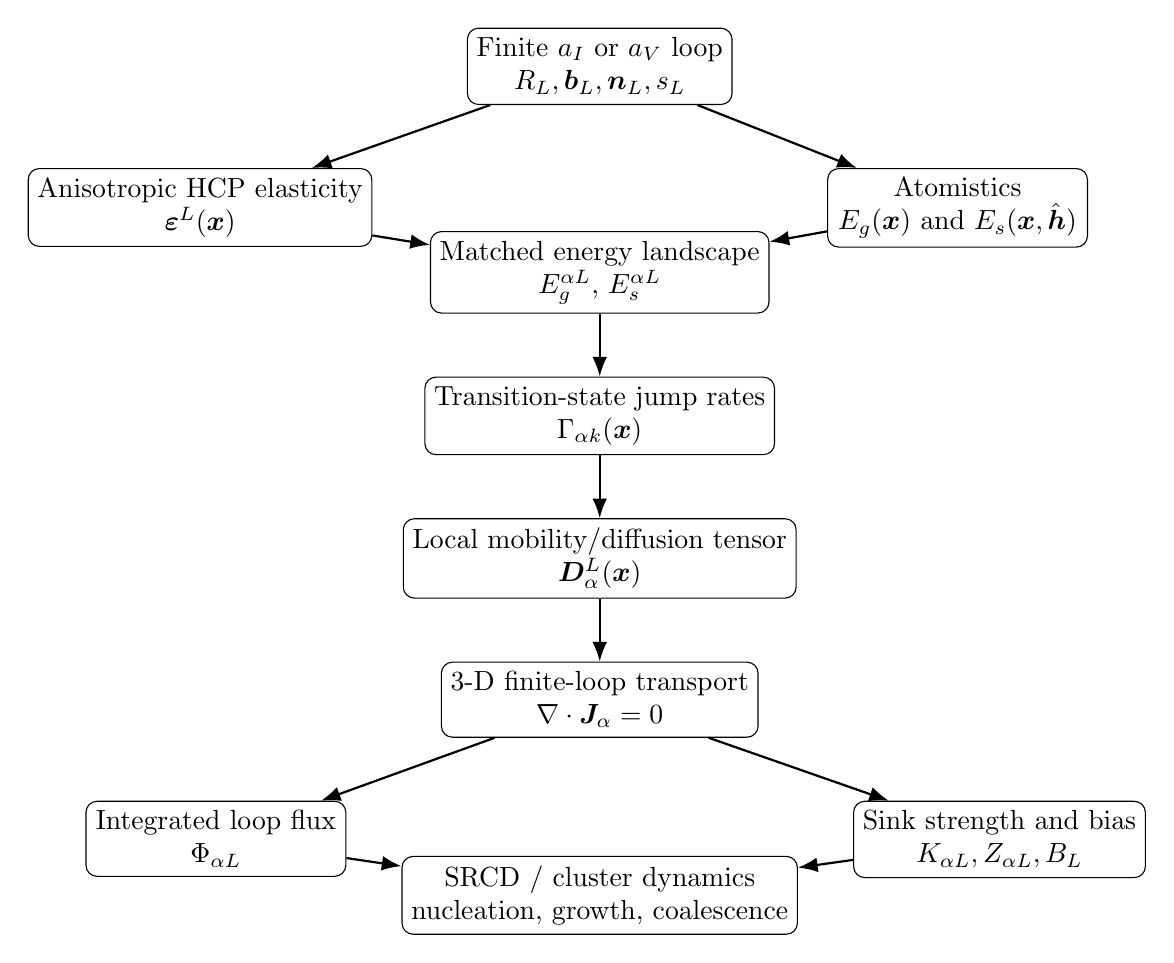
\begin{tikzpicture}[
node distance=8mm and 12mm,
box/.style={draw,rounded corners,align=center,minimum width=3.3cm,minimum height=0.9cm},
arrow/.style={-{Latex[length=2.5mm]},thick}]
\node[box] (loop) {Finite $a_I$ or $a_V$ loop\\$R_L,\bb_L,\bn_L,s_L$};
\node[box,below left=of loop] (elastic) {Anisotropic HCP elasticity\\$\beps^L(\bx)$};
\node[box,below right=of loop] (atom) {Atomistics\\$E_g(\bx)$ and $E_s(\bx,\hat{\bh})$};
\node[box,below=16mm of loop] (energies) {Matched energy landscape\\$E_g^{\alpha L}$, $E_s^{\alpha L}$};
\node[box,below=of energies] (rates) {Transition-state jump rates\\$\Gamma_{\alpha k}(\bx)$};
\node[box,below=of rates] (diff) {Local mobility/diffusion tensor\\$\bD_\alpha^L(\bx)$};
\node[box,below=of diff] (pde) {3-D finite-loop transport\\$\nabla\cdot\bJ_\alpha=0$};
\node[box,below left=of pde] (flux) {Integrated loop flux\\$\Phi_{\alpha L}$};
\node[box,below right=of pde] (bias) {Sink strength and bias\\$K_{\alpha L},Z_{\alpha L},B_L$};
\node[box,below=15mm of pde] (srcd) {SRCD / cluster dynamics\\nucleation, growth, coalescence};
\draw[arrow] (loop)--(elastic);\draw[arrow] (loop)--(atom);
\draw[arrow] (elastic)--(energies);\draw[arrow] (atom)--(energies);
\draw[arrow] (energies)--(rates);\draw[arrow] (rates)--(diff);\draw[arrow] (diff)--(pde);
\draw[arrow] (pde)--(flux);\draw[arrow] (pde)--(bias);\draw[arrow] (flux)--(srcd);\draw[arrow] (bias)--(srcd);
\end{tikzpicture}
\end{center}

\section{Conclusions}
A physically complete finite-loop bias calculation for irradiated $\alpha$-Zr should solve point-defect transport around the actual finite loop rather than assign a fixed empirical bias. The recommended structure is
\begin{equation}
\boxed{
\begin{array}{c}
\text{finite-loop anisotropic elastic field}\\
\downarrow\\
E_g^{\alpha L}(\bx),\;E_s^{\alpha L}(\bx,\hat{\bh})\\
\downarrow\\
\Gamma_{\alpha k}(\bx),\;\bD_\alpha^L(\bx)\\
\downarrow\\
\nabla\cdot\{\bD_\alpha^L[\nabla C_\alpha+\beta C_\alpha\nabla E_g^{\alpha L}]\}=0\\
\downarrow\\
\Phi_{\alpha L}\rightarrow K_{\alpha L}\rightarrow Z_{\alpha L}\rightarrow B_L\rightarrow\dot R_L.
\end{array}}
\end{equation}
The formulation contains classical isotropic elastic bias, Woo's saddle-point anisotropy, HCP diffusion anisotropy, and March-Rico-type atomistic loop binding as controlled limits of the same transport problem. The most important new atomistic input required for a decisive comparison is the spatially resolved saddle-point energy landscape around finite vacancy and interstitial $a$-loops.

\begin{thebibliography}{99}
\bibitem{Woo1981} C.~H. Woo, ``The sink strength of a dislocation loop in the effective medium approximation,'' \emph{Journal of Nuclear Materials} 98 (1981) 279--294. doi:10.1016/0022-3115(81)90154-9.
\bibitem{Woo1982} C.~H. Woo, ``Intrinsic bias differential between vacancy loops and interstitial loops,'' \emph{Journal of Nuclear Materials} 107 (1982) 20--30. doi:10.1016/0022-3115(82)90555-4.
\bibitem{DederichsSchroeder1978} P.~H. Dederichs and K. Schroeder, ``Anisotropic diffusion in stress fields,'' \emph{Physical Review B} 17 (1978) 2524--2536. doi:10.1103/PhysRevB.17.2524.
\bibitem{SchroederDettmann1975} K. Schroeder and K. Dettmann, ``Diffusion reactions in long range potentials,'' \emph{Zeitschrift f\"ur Physik B} 22 (1975) 343--350. doi:10.1007/BF01312804.
\bibitem{BrailsfordBulloughHayns1976} A.~D. Brailsford, R. Bullough, and M.~R. Hayns, ``Point defect sink strengths and void-swelling,'' \emph{Journal of Nuclear Materials} 60 (1976) 246--256. doi:10.1016/0022-3115(76)90139-2.
\bibitem{BulloughHaynsWoo1979} R. Bullough, M.~R. Hayns, and C.~H. Woo, ``The sink strength of dislocation loops and their growth in irradiated materials,'' \emph{Journal of Nuclear Materials} 84 (1979) 93--100. doi:10.1016/0022-3115(79)90152-1.
\bibitem{MarchRicoWirth2023} J.~F. March-Rico and B.~D. Wirth, ``Stress states and point defect capture radii of dislocation $a$-loops and $c$-loops in alpha-zirconium,'' \emph{Journal of Nuclear Materials} 587 (2023) 154752. doi:10.1016/j.jnucmat.2023.154752.
\bibitem{MarchRicoBlondelWirth2025} J.~F. March-Rico, S. Blondel, and B.~D. Wirth, ``Atomistically-informed cluster dynamics modeling of concurrent interstitial and vacancy $a$-loop evolution in irradiated alpha-zirconium,'' \emph{Acta Materialia} 288 (2025) 120777. doi:10.1016/j.actamat.2025.120777.
\bibitem{Chulkin2008} D.~A. Chulkin, V.~M. Chernov, and A.~B. Sivak, ``Self-point defects characteristics and their dependence on stress fields of edge and screw basal dislocations with Burgers vector $1/3\langle11\bar20\rangle$ in HCP Zr,'' \emph{AIP Conference Proceedings} 999 (2008) 146--156. doi:10.1063/1.2918101.
\bibitem{HirthLothe} J.~P. Hirth and J. Lothe, \emph{Theory of Dislocations}, 2nd ed., Wiley, New York, 1982.
\bibitem{Mura} T. Mura, \emph{Micromechanics of Defects in Solids}, 2nd ed., Martinus Nijhoff, Dordrecht, 1987.
\bibitem{BarattaFEniCSx} I.~A. Baratta, J.~P. Dean, J.~S. Dokken, M. Habera, J.~S. Hale, C.~N. Richardson, M.~E. Rognes, M.~W. Scroggs, N. Sime, and G.~N. Wells, ``DOLFINx: The next generation FEniCS problem solving environment,'' 2023. doi:10.5281/zenodo.10447666.
\bibitem{AlnaesUFL} M.~S. Aln{\ae}s, A. Logg, K.~B. {\O}lgaard, M.~E. Rognes, and G.~N. Wells, ``Unified Form Language: A domain-specific language for weak formulations of partial differential equations,'' \emph{ACM Transactions on Mathematical Software} 40 (2014). doi:10.1145/2566630.
\bibitem{GastonMOOSE} D. Gaston, C. Newman, G. Hansen, and D. Lebrun-Grandi\'e, ``MOOSE: A parallel computational framework for coupled systems of nonlinear equations,'' \emph{Nuclear Engineering and Design} 239 (2009) 1768--1778. doi:10.1016/j.nucengdes.2009.05.021.
\bibitem{PermannMOOSE} C.~J. Permann, D.~R. Gaston, D. Andr\v{s}, R.~W. Carlsen, F. Kong, A.~D. Lindsay, J.~M. Miller, J.~W. Peterson, A.~E. Slaughter, R.~H. Stogner, and R.~C. Martineau, ``MOOSE: Enabling massively parallel multiphysics simulation,'' \emph{SoftwareX} 11 (2020) 100430. doi:10.1016/j.softx.2020.100430.
\bibitem{ScharfetterGummel} D.~L. Scharfetter and H.~K. Gummel, ``Large-signal analysis of a silicon Read diode oscillator,'' \emph{IEEE Transactions on Electron Devices} 16 (1969) 64--77. doi:10.1109/T-ED.1969.16566.
\bibitem{MalerbaBecquartDomain2007} L. Malerba, C.~S. Becquart, and C. Domain, ``Object kinetic Monte Carlo study of sink strengths,'' \emph{Journal of Nuclear Materials} 360 (2007) 159--169. doi:10.1016/j.jnucmat.2006.10.002.
\end{thebibliography}
\end{document}
